% This document is part of the GaussianProductRefactor project.
% Copyright 2019, 2020 the authors. All rights reserved.

% to-do
% -----
% - audit all style notes
% - fix typesetting for "canonical form" of normal
% - APW: update links to data files when archived with Zenodo
% - HOGG: audit terms defined in quotation marks; should we use \textsl instead?
% - HOGG: Audit all N K etc. It's a mess. And there have been HUGE errors.
% - HOGG: Check Gaussian Processes literature for a relevant thing to cite
% - HOGG: cite Rasmussen, Matrix cookbook, Roweis notes
% - HOGG: Refer to Luger, F-M, Hogg RNAAS? https://arxiv.org/pdf/1710.11136.pdf
% - APW: We mention SPEED of computation in the abstract; we should say that again
%   in the introduction and parts of the conversation below it. Refer to
%   The Joker appropriately. THERE NEED TO BE CITATIONS! ArXiv rejects papers that
%   don't have bibliographies.
% - WE NEED TO GIVE THE FORM FOR A GAUSSIAN!! WE DON'T GIVE THAT.
% - make a comment about the connection to GPs, and what it means.
% - audit for and remove all HOGG, DWH, APW, BL, CITE from the text.
% - send to friendlies (DFM, Lang, Bovy, Rix, others??)
% - post to arXiv
% - profit

% style notes -- audit for these.
% -------------------------------
% - use \, for multiplication
% - put punctuation after equations as necessary, with "~," or equivalent. Use ~
% - no condescending language; no "it is easy to show" or equivalent...!
% - use \vA not A or \vector{A} and so on.
% - modify typesetting above the \begin{document} line, not below.
% - distinguish types (vector, matrix, tensor).
% - never say ``the pdf for $\vy$''; instead say ``the pdf for the data $\vy$''.
% - put term name definitions in \textsl{}, *not* quotations
% - nonlinear not non-linear
% - don't say "i.e.," say "that is,". Don't say "e.g.," say "for example,".
% - ...[your pet peeve here]...

\documentclass[12pt, letterpaper]{article}
\usepackage{amsmath, bm, mathrsfs, amssymb}
\usepackage[dvipsnames]{xcolor}
\usepackage[hidelinks,
            colorlinks=true,
            linkcolor=black,
            urlcolor=CornflowerBlue]{hyperref}
\usepackage{pifont}
\usepackage{graphicx}

\usepackage{caption}
\captionsetup{font=footnotesize}

% text stuhh
\newcommand{\documentname}{\textsl{Note}}
\newcommand{\sectionname}{Section}
\newcommand{\equationname}{equation}
\renewcommand{\tablename}{Table}
\newcommand{\acronym}[1]{{\small{#1}}}
\newcommand{\code}[1]{\texttt{#1}}
\newcommand{\foreign}[1]{\textsl{#1}}

% math stuhh
\newcommand{\given}{\,|\,}
\newcommand{\dd}{\mathrm{d}}
\newcommand{\T}{^{\!\mathsf{T}\!}}
\newcommand{\inv}{^{-1}}
\newcommand{\scalar}[1]{#1}
\renewcommand{\vector}[1]{\boldsymbol{#1}}
\newcommand{\tensor}[1]{\mathbf{#1}}
\renewcommand{\matrix}[1]{\mathsf{#1}}
\newcommand{\normal}{\mathcal{N}\!\,}

% variables
\newcommand{\va}{\vector{a}}
\newcommand{\vb}{\vector{b}}
\newcommand{\vm}{\vector{m}}
\newcommand{\vx}{\vector{x}}
\newcommand{\vy}{\vector{y}}
\newcommand{\vz}{\vector{z}}
\newcommand{\vmu}{\vector{\mu}}
\newcommand{\veta}{\vector{\eta}}
\newcommand{\vtheta}{\vector{\theta}}
\newcommand{\tA}{\tensor{A}}
\newcommand{\tB}{\tensor{B}}
\newcommand{\tC}{\tensor{C}}
\newcommand{\tD}{\tensor{D}}
\newcommand{\tI}{\tensor{I}}
\newcommand{\tQ}{\tensor{Q}}
\newcommand{\tS}{\tensor{S}}
\newcommand{\tH}{\tensor{H}}
\newcommand{\tV}{\tensor{V}}
\newcommand{\tLambda}{\tensor{\Lambda}}
\newcommand{\mM}{\matrix{M}}
\newcommand{\mN}{\matrix{N}}
\newcommand{\mU}{\matrix{U}}
\newcommand{\mV}{\matrix{V}}
\newcommand{\bP}{\ensuremath{\textrm{\ding{80}}}} % THIS IS HERE TO ANNOY DWH / you failed
\newcommand{\bH}{\ensuremath{\textrm{\ding{114}}}} % THIS IS HERE TO ANNOY DWH / you failed

% typesetting stuff
\addtolength{\topmargin}{-0.75in}
\addtolength{\textheight}{1.5in}
\setlength{\parindent}{\baselineskip}
\raggedbottom\sloppy\sloppypar\frenchspacing

\usepackage{color}
\newcommand{\todo}[1]{\textcolor{BrickRed}{[TODO: #1]}}
\newcommand{\bl}[1]{\textcolor{red}{[BL says: #1]}}
\newcommand{\hogg}[1]{\textcolor{magenta}{[Hogg says: #1]}}

\begin{document}

\section*{Data Analysis Recipes:\\ Products of dependent multivariate Gaussians}

\noindent\textbf{David W. Hogg}\footnote{%
The authors would like to thank
  Dan Foreman-Mackey (Flatiron) and
  Sam Roweis (deceased),
for help with all these concepts through the years.
This work was supported in part by the National Science Foundation
and the National Aeronautics and Space Administration. It was developed
in part at \textsl{AstroHackWeek 2016}, which was hosted at Berkeley
by the Moore--Sloan Data Science Environment.
}\\
{\footnotesize%
  \textsl{Center for Cosmology and Particle Physics, Department of Physics, New York University}\\
  \textsl{Max-Planck-Institut f\"ur Astronomie, Heidelberg}\\
  \textsl{Flatiron Institute, a division of the Simons Foundation}%
}

\medskip\noindent\textbf{Adrian~M.~Price-Whelan}\\
{\footnotesize%
  \textsl{Flatiron Institute, a division of the Simons Foundation}%
}

\medskip\noindent\textbf{Boris Leistedt}\\
{\footnotesize%
  \textsl{Department of Physics, Imperial College, London}\\
  \textsl{Center for Cosmology and Particle Physics, Department of Physics, New York University}%
}

\paragraph{Abstract:}
A product of two Gaussians---or normal distributions---is another Gaussian.
That's a valuable and useful fact!
Here we use it to derive a refactoring of a common product of
multivariate Gaussians:
The product of a Gaussian likelihood times a Gaussian prior, where some or all
of those parameters enter the likelihood only in the mean and only linearly.
That is, a linear, Gaussian model.
This product of a likelihood times a prior can be refactored into a product of a
Bayesian evidence (or marginalized likelihood) times a posterior, where
(in this case) both of these are also Gaussian.
The means and variance tensors of the refactored Gaussians are straightforward
to obtain as closed-form expressions;
here we deliver these expressions, with discussion.
The closed-form expressions can be used to speed up and improve the precision
of inferences that contain linear parameters with Gaussian priors.
We connect the methods to inferences that arise frequently in physics
and astronomy.

If all you want is the answer, the question is posed and answered at the
beginning of \sectionname~\ref{sec:problemsolution}, and a generalization to
products of many Gaussians is given in \sectionname~\ref{sec:generalization}.
We show two toy examples, in the form of worked exercises, in
\sectionname~\ref{sec:examples}.


\section{Inferences with linear parameters}

It is common in physics and astronomy and engineering and machine learning and many other fields that likelihood functions
(probabilities of data given parameters) are chosen to be Gaussian
(or normal\footnote{In this \documentname, we obey physics and astronomy
  conventions and refer to the normal pdf as the Gaussian pdf. We apologize;
  we realize that it is dumb and inaccurate to name things after people when
  those things also have generic, descriptive names.
  On the other hand, ``normal'' isn't the finest
  name either. Perhaps Gaussian pdfs should be called ``central'' since they are
  produced by the central limit theorem. Anyway, we will continue with
  the name ``Gaussian'' despite our own reservations. Apologies.}):
One reason is that a likelihood function is basically a noise model,
and it is often case that the noise is treated as Gaussian.
This Gaussian assumption for the likelihood function is
\emph{accurate} when the noise model has benefitted from the central
limit theorem.
This is true, for example, when the noise is thermal, or when the
noise is shot noise and the numbers (numbers of detected photons or other
particles) are large.
Another reason that the likelihood function is often treated as
Gaussian is that Gaussians are generally \emph{tractable}:
Many computations we like to perform on Gaussians, like integrals and
derivatives and optimizations, have closed-form solutions.
Even when we don't use the closed-form solutions, there are many
contexts in which Gaussians lead to convex optimizations,
providing guarantees to resulting inferences.

It is also common in physics and astronomy that models for data
include parameters such that the expectation value for the data (in,
say, a set of repeated experiments) is linearly proportional to some
subset of the parameters.
This is true, for example, when we fit a histogram of \textsl{Large Hadron Collider}
events
affected by the Higgs boson\footnote{See, for example, HOGG CITE};
the expected number of counts in each
energy bin is proportional to a linear combination of the amplitudes
of various backgrounds and some coupling to the Higgs.
This is true, for example, when we fit for the radial-velocity
variation of a star in response to an faint, orbiting companion\footnote{See,
  for an example in our own work, APW CITE JOKER. That project and paper would have been
  impossible without the speed-ups provided by the expressions derived in this
  \documentname.} (this is a context
we will use for one of our toy examples below), where the expectation of the
radial-velocity measurements depends linearly on the binary system
velocity and some combination of masses and system inclination (with
respect to the line of sight).
In both of these cases, there are both linear parameters (like the
amplitudes) and nonlinear parameters (like the mass of the Higgs, or
the orbital period of the binary).
In what follows, we will spend our energies on the linear parameters,
though our work on them is in service of learning the nonlinear
parameters too, of course.

Bayes theorem is often written as a ratio of probability density
functions (pdfs in what follows), but it can be written as a simple
pdf factorization:
\begin{equation}
p(\vy,\vtheta\given\bH) = p(\vy\given\vtheta,\bH)\,p(\vtheta\given\bH) = p(\vtheta\given\vy,\bH)\,p(\vy\given\bH)
\end{equation}
where
$p(\vy,\vtheta\given\bH)$ is the joint probability of data $\vy$ and
parameters $\vtheta$ given your model assumptions and hyper parameters
(symbolized jointly as $\bH$)\footnote{%
\textsl{Typographical note:} In this \documentname, we
typeset vectors (which are column vectors) as $\va, \vb, \vtheta$, we typeset tensors (which
are square, non-negative semi-definite matrices) as $\tC, \tLambda$,
we typeset matrices (which will in general be non-square) as $\mM, \mU$,
and we typeset blobs or unstructured
collections of information as $\bH, \bP$.},
$p(\vy\given\vtheta,\bH)$ is the likelihood, or probability of data $\vy$
given parameters (and assumptions),
$p(\vtheta\given\bH)$ is the prior pdf for the parameters $\vtheta$,
$p(\vtheta\given\vy,\bH)$ is the posterior pdf for the parameters $\vtheta$
given the data,
and
$p(\vy\given\bH)$ is the pdf for the data, marginalizing out all of the linear
parameters (hereafter, we refer to this as the \textsl{marginalized
likelihood}\footnote{In the case that the problem has no parameters other than
the linear parameters $\vtheta$, this term, $p(\vy \given \bH)$, is sometimes
called the \textsl{Bayesian evidence} or the \textsl{fully marginalized
likelihood}.}).

If the likelihood is Gaussian, and the expectation of the data depends linearly
on the parameters, and if we choose the prior pdf to also be Gaussian, then
everything else (the joint, the posterior, and the marginalized likelihood)
becomes Gaussian too.
The main point of this \documentname\ is that the means and variances of these
five Gaussians are all related by simple, closed-form expressions, given below.
One consequence of this math is that \emph{if} you have a Gaussian
likelihood function, and \emph{if} you have a subset of parameters that are
linearly related to the expectation of the data, \emph{then} you can obtain both
the posterior pdf $p(\vtheta\given\vy,\bH)$ and the marginalized likelihood
$p(\vy\given\bH)$ with closed-form transformations of the means and variances of
the likelihood and prior pdf.

\section{Marginalization by refactorization}

Imagine that we are doing an inference using data $\vy$ (which is a
$N$-dimensional vector, say).
We are trying to learn linear parameters $\vtheta$ (a $K$-dimensional vector)
and also nonlinear parameters $\bP$ (an arbitrary vector, list, or
blob).\footnote{Here, $\bP$ represents the nonlinear parameters \emph{and}
assumptions or hyper parameters.}
Whether we are Bayesian or frequentist, the inference is based on
a likelihood function, or probability for the data given parameters
\begin{equation}
\mbox{likelihood} \quad p(\vy\given\vtheta,\bP) ~ .
\end{equation}

Now let's imagine that the parameters $\vtheta$ are either nuisance
parameters, or else easily marginalized, so we want to marginalize
them out.
This will leave us with a lower-dimensional marginalized likelihood
function
\begin{equation}
\mbox{marginalized likelihood} \quad p(\vy\given\bP) ~ .
\end{equation}
That's good, but the marginalization comes at a cost:
We have to choose a prior
\begin{equation}
\mbox{prior on nuisance parameters} \quad p(\vtheta\given\bP)
\end{equation}
on the nuisances.
This is the basis for the claim (stated elsewhere; HOGG) that
inference requires a likelihood function, and priors on the nuisance parameters.
It does not require a prior on everything, contrary to some statements
in the pedagogical literature (for example, HOGG).
We have said ``$p(\vtheta\given\bP)$'' because this prior may depend on
the nonlinear parameters $\bP$, but it certainly doesn't have to.

To perform the marginalization, we have two choices.
We can either do an integral:
\begin{equation}
p(\vy\given\bP) = \int p(\vy\given\vtheta,\bP)\,p(\vtheta\given\bP)\,\dd\vtheta
~ ,
\end{equation}
where the integral is implicitly over the entire domain of the
nuisances $\vtheta$ (or the entire support of the prior).
Or we can re-factorize the expression using Bayes' theorem:
\begin{equation}
p(\vy\given\vtheta,\bP)\,p(\vtheta\given\bP)
 = p(\vtheta\given\vy,\bP)\,p(\vy\given\bP)
~ .
\end{equation}
That is, in certain magical circumstances it is possible to do this
re-factorization without explicitly doing any integral.
When this is true, the marginalization is sometimes far easier than
the relevant integral.

One such magical circumstance can arise when the two probability
distributions---the likelihood and the prior---are both Gaussian in
form, and when the model is linear.
In detail we will assume
\begin{enumerate}
\item
the likelihood $p(\vy\given\vtheta,\bP)$ is a Gaussian in $\vy$,
\item
the prior $p(\vtheta\given\bP)$ is a Gaussian in $\vtheta$,
\item
the mean of the likelihood Gaussian depends linearly on the nuisance
parameters $\vtheta$, and
\item
the nuisance parameters $\vtheta$ don't enter the likelihood anywhere
other than in the mean.
\end{enumerate}
In equations, this becomes:
\begin{equation}
p(\vy\given\vtheta,\bP) = \normal(\vy\given\mM\cdot\vtheta,\tC)
\end{equation}
\begin{equation}
p(\vtheta\given\bP) = \normal(\vtheta\given\vmu,\tLambda)
~ ,
\end{equation}
where
$\normal(\vx\given\vm,\tV)$ is the multivariate Gaussian pdf for a vector $\vx$
given a mean vector $\vm$ and a variance tensor $\tV$,
$\mM$ is a $N\times K$ rectangular design matrix (which depends, in
general, on the nonlinear parameters $\bP$),
$\tC$ is a $N\times N$ covariance matrix of uncertainties for the
data (diagonal if the data dimensions are independent).
That is, the likelihood is a Gaussian with a mean that depends
linearly on the nuisance parameters $\vtheta$, and
$\vmu$ and $\tLambda$ are the $K$-vector mean and $K\times K$ variance tensor
for the Gaussian prior.

In this incredibly restrictive---but also surprisingly
common---situation, the re-factored pdfs $p(\vtheta\given\vy,\bP)$
(also known as the posterior for the linear parameters, conditioned on
the nonlinear parameters in $\bP$) and $p(\vy\given\bP)$ (the
partially marginalized likelihood, marginalizing out the linear
parameters) will also both be Gaussian.
Obtaining the specific forms of these Gaussians is the object of this
\documentname.

\section{Products of two Gaussians}\label{sec:problemsolution}

On the internets, there are many documents, slide decks, and videos
that explain products of Gaussians in terms of other Gaussians.
The vast majority of these consider either the univariate case (where
the data $\vy$ and the parameter $\vtheta$ are both simple scalars, which
is not useful for our science cases), or the same-dimension case (where the data
$\vy$ and the parameter vector $\vtheta$ are the same length, which never
occurs in our applications).
Here we solve this problem in the general case:
The inputs are multivariate (vectors) and the two Gaussians we are
multiplying live in spaces of different dimensions.
That is, we solve the following problem:

\paragraph{Problem:}
Find $K$-vector $\va$, $K\times K$ variance tensor $\tA$, $N$-vector $\vb$,
and $N\times N$ variance tensor $\tB$ such that
\begin{equation}\label{eq:problem}
\normal(\vy\given\mM\cdot\vtheta,\tC)\,\normal(\vtheta\given\vmu,\tLambda)
 = \normal(\vtheta\given\va,\tA)\,\normal(\vy\given\vb,\tB) ~ ,
\end{equation}
and such that $\va$, $\tA$, $\vb$, and $\tB$ don't depend on $\vtheta$ at all.
Note that
$\vy$ is a $N$-vector,
$\mM$ is a $N\times K$ matrix,
$\vtheta$ is a $K$-vector,
$\tC$ is a $N\times N$ non-negative semi-definite variance tensor,
$\vmu$ is a $K$-vector,
and
$\tLambda$ is a $K\times K$ non-negative semi-definite variance tensor.

\paragraph{Solution:}
\begin{equation}\label{eq:A}
\tA\inv = \tLambda\inv + \mM\T \cdot \tC\inv \cdot \mM
\end{equation}
\begin{equation}\label{eq:a}
\va = \tA \cdot (\tLambda\inv \cdot \vmu + \mM\T \cdot \tC\inv \cdot \vy)
\end{equation}
\begin{equation}\label{eq:B}
\tB = \tC + \mM \cdot \tLambda \cdot \mM\T
\end{equation}
\begin{equation}\label{eq:b}
\vb = \mM \cdot \vmu
~ .
\end{equation}
This is the complete solution to the problem, and constitutes the main point
of this \documentname.
For completeness, we will give some discussion!

\paragraph{Proof:}
The two sides of \equationname~(\ref{eq:problem}) are identical if two things
hold.
The first thing is that the determinant products must be equal:
\begin{equation}
||\tC||\,||\tLambda|| = ||\tA||\,||\tB||
~ ,
\end{equation}
because the determinants are involved in the normalizations of the
functions.
This equality of determinant products follows straightforwardly from
the matrix determinant lemma (APW CITE WIKIPEDIA OR ??)
\begin{equation}\label{eq:detlemma}
||\tQ + \mU\cdot\mV\T|| = ||\tI + \mV\T\cdot\tQ\inv\cdot\mU||\,||\tQ||
~ ,
\end{equation}
where $\mU$ and $\mV$ can be rectangular, and $\tI$ is the correct-sized identity matrix.
This identity implies that
\begin{equation}
||\tA\inv|| = ||\tI + \mM\T\cdot\tC\inv\cdot\mM\cdot\tLambda||\,||\tLambda\inv||
\end{equation}
\begin{equation}
||\tB||     = ||\tI + \mM\T\cdot\tC\inv\cdot\mM\cdot\tLambda||\,||\tC||
~,
\end{equation}
where we had to apply the identity twice to get the $||\tA\inv||$ expression.
We can ratio these as follows to prove this first thing:
\begin{equation}
||\tA||\,||\tB||
 = \frac{||\tB||}{||\tA\inv||}
 = \frac{||\tC||}{||\tLambda\inv||}
 = ||\tC||\,||\tLambda||
~ .
\end{equation}

The second thing required for the proof is that the quadratic scalar form
\begin{equation}\label{eq:LHS}
[\vy-\mM\cdot\vtheta]\T\cdot\tC\inv\cdot[\vy-\mM\cdot\vtheta]
+ [\vtheta-\vmu]\T\cdot\tLambda\inv\cdot[\vtheta-\vmu]
\end{equation}
must equal the quadratic scalar form
\begin{equation}\label{eq:RHS}
[\vtheta-\va]\T\cdot\tA\inv\cdot[\vtheta-\va]
+ [\vy-\vb]\T\cdot\tB\inv\cdot[\vy-\vb]
~,
\end{equation}
because these quadratic scalar forms appear in the exponents in the functions.
This equality follows from straightforward expansion of
all the quadratic forms, plus some use of the matrix inversion lemma
(APW CITE WIKIPEDIA OR ??),
\begin{equation}\label{eq:invlemma}
[\tQ + \mU\cdot\tS\cdot\mV\T]\inv = \tQ\inv - \tQ\inv\cdot\mU\cdot[\tS\inv + \mV\T\cdot\tQ\inv\cdot\mU]\inv\cdot\mV\T\cdot\tQ\inv
~ ,
\end{equation}
which gives an expression for the inverse $\tB\inv$ of the marginalized
likelihood variance:
\begin{equation}
\tB\inv = \tC\inv - \tC\inv\cdot\mM\cdot[\tLambda\inv + \mM\T\cdot\tC\inv\cdot\mM]\inv\cdot\mM\T\cdot\tC\inv
~ .
\end{equation}
After that it's just a lot of grinding through matrix expressions.\footnote{%
We leave this grinding to the avid reader.
For guidance, it might help to realize that there are terms that
contain $\vtheta\T\cdots\vtheta$, $\vtheta\T\cdots\vy$, $\vy\T\cdots\vy$,
$\vtheta\T\cdots\vmu$, and $\vmu\T\cdots\vmu$.
If you expand out each of these five kinds of terms, each of the five
should lead to an independent-ish equality.}

\paragraph{Solution notes:}
In principle we found this factorization by expanding the quadratic in
(\ref{eq:LHS}) and then completing the square.
Of course we didn't really; we used arguments (which physicists love)
called \emph{detailed balance}:
We required that the terms that look like
$\vtheta\T\cdot\tQ\cdot\vtheta$ were equal between the LHS~(\ref{eq:LHS})
and the RHS~(\ref{eq:RHS}), and then all the terms that look like
$\vmu\T\cdot\tS\cdot\vmu$, and so on.
It turns out you don't have to consider them all to get the right solution.

Because the matrix $\mM$ is not square, it has no inverse. And because this
is a physics problem, it has units (which are the units of $\dd\vy/\dd\vtheta$).
It's beautiful in the solution that $\mM$ and $\mM\T$ appear only where the
units make sense.
They make sense because the units of $\tC\inv$ are inverse data-squared (where $\vy$
is the data vector) and the units of $\tLambda$ are parameters-squared and the units
of $\mM$ are data over parameters.
And they are all different sizes.

Various parts of the solution are highly interpretable in terms of the
objects of Bayesian inference. For example, because the term $p(\vtheta\given \va,\tA)$
is the conditional
posterior pdf for the linear parameters $\vtheta$, the vector $\va$ is the
maximum \foreign{a posteriori} (or \acronym{MAP}) value for the parameter vector
$\vtheta$.
It is found by inverse-variance-weighted combinations of the data and the prior.
In some projects posterior pdfs or \acronym{MAP} parameter values are the goal
(although we don't think it often should be\footnote{HOGG WRITE STUFF ABOUT WHY YOU WANT TO PUBLISH LFs and marginalized LFs.}); these expressions deliver the posterior
straightforwardly too.
The variance tensor $\tA$ is the posterior variance in the parameter space.
It is strictly non-larger (in eigenvalues or determinant) than either
the prior variance $\tLambda$ or the parameter-space data-noise
variance $\mM\T\cdot\tC\cdot\mM$.
The vector $\vb$ is the prior-optimal (maximum \foreign{a priori})
value for the data $\vy$.
It is the most likely data vector, and also the expectation for the data,
under the prior pdf.
And the variance tensor $\tB$ is the prior variance expanded out to the
data space, and including the noise variance in the data.
It is strictly non-smaller than both the data noise variance $\tC$ and the
data-space prior variance $\mM\cdot\tLambda\cdot\mM\T$.

\paragraph{Implementation notes:}
The solution gives an expression for the variance tensor $\tB$, but
note that when you actually evaluate the pdfs you probably need to
have either the inverse of $\tB$, or else an operator that computes
the product of the inverse and vectors, as in $\tB\inv\cdot\vy$ and
the same for $\vb$.
To get the inverse of the tensor $\tB$ stably, \emph{you might want to use
the matrix inversion lemma} (\ref{eq:invlemma}) given above.
This is often useful because you often know the data noise-variance
tensor inverse $\tC\inv$, and the prior variance inverse
$\tLambda\inv$, and the lemma manipulates these into the answer without
any heavy linear algebra.
The lemma saves you the most time and precision when the parameter size $K$
is much smaller than the data size $N$ (or vice versa); that is, when $\mM$
is ``very non-square''.

We also give the general advice that one should \emph{never take an explicit
inverse} (unless you know the inverse exactly in closed form, as you do
for, say, diagonal tensors).
In your code you should never use the \code{inv()} function; you
should always use a \code{solve()} function.
The reason is that the code operation \code{inv(B)} returns the best
possible inverse to machine precision (if you are lucky), but what you
really want instead is the best possible product of that inverse times
a vector.
So in general \code{solve(B,y)} will deliver more precise results than
the mathematically equivalent \code{dot(inv(B),y)}.

The expressions in (\ref{eq:problem}) do not require that the tensors
$\tC$, $\tLambda$, $\tA$, $\tB$ be positive definite; they only require
that they be non-negative semi-definite.
That means that they can have zero eigenvalues.
As can their inverses $\tC\inv$, $\tLambda\inv$, $\tA\inv$, $\tB\inv$.
If either of these might happen in your problem---like if your prior
freezes the parameters to a subspace of the $\vtheta$-space, which
would lead to a zero eigenvalue in $\tLambda$, or if a data point is
unmeasured or missing, which would lead to a zero eigenvalue in
$\tC\inv$---you might have to \emph{think about how you implement the
  linear algebra operations to be zero-safe}\footnote{HOGG: WRITE SOMETHING
  here about what it looks like when, say, $\tA$ or $\tB$ contains
  zero eigenvalues. It leads to directions in $\vtheta$ or $\vy$ space
  in which log probabilities are negative-infinity. These are
  disallowed directions. In this world, data and parameters \emph{are
    not permitted} to go in those directions. What does ``zero-safe''
  look like in this context?}.


\paragraph{Simplification: single multiplicative scaling}

One interesting case is when $K=1$, so the design matrix in fact
reduces to a model vector $\vm$, multiplied by a scalar $\theta$, and
$\mu$ and $\Lambda$ are now scalars as well:
\begin{equation}
\mbox{likelihood} \times \mbox{prior} \quad \normal(\vy\given\theta\,\vm,\tC)\,\normal(\theta\given\mu,\Lambda) = \normal(\theta\given a,A)\,\normal(\vy\given\vb,\tB)
~ .
\end{equation}
In this case, the previous equations are simplified and no longer
involve many matrix operations. It's a nice exercise to simplify the
solution above for this scalar case.


\section{Worked Examples}\label{sec:examples}

When working with a probabilistic model that meets the strong requirements
imposed above (Gaussians everywhere; expectations linear in parameters),
the identities described in this
\documentname\ have practical uses: (1) To simplify the posterior pdf of your
model (which makes generating samples or computing integrals far simpler), and
(2) to reduce the dimensionality of your model (by enabling closed-form
marginalizations over linear parameters).
Reducing the dimensionality of your parameter-space will in general improve
convergence of Markov Chain Monte Carlo\footnote{We have also written a tutorial
  on MCMC in this series (APW CITE HOGG \& DFM).} (MCMC)
sampling methods, or enable
alternate sampling methods (for example, rejection sampling) that may be intractable
when the parameter dimensionality is large.

Here, we demonstrate the utility of the identities shown above with two toy,
worked exercises: The examples are written such that the problems are set up
first, and the solutions are given below.


\subsection{Exercise 1: A fully linear model}

\paragraph{Problem:} We observe a set of data $(x_i, y_i)$ (indexed by $i$) with
known, Gaussian uncertainties in $y$, $\sigma_{y_i}$, and no uncertainty in $x$.
\todo{Connect this to centroiding peaks in spectroscopy or whatever - give it negative curvature}
The parametric model we will use for this data is a quadratic polynomial,
\begin{equation}
  % APW: I used greek here because a, b are used in expressions above...
  f(x \,;\, \alpha, \beta, \gamma) = \alpha\,x^2 + \beta\,x + \gamma
\end{equation}
and we assume we have Gaussian prior pdfs on all of the parameters $(\alpha,
\beta, \gamma)$,
\begin{align}
  p(\alpha) &= \normal(\alpha \given \mu_\alpha, \sigma_\alpha)\\
  p(\beta) &= \normal(\beta \given \mu_\beta, \sigma_\beta)\\
  p(\gamma) &= \normal(\gamma \given \mu_\gamma, \sigma_\gamma)
  ~ .
\end{align}

\tablename~\ref{tbl:data1} contains four data points, $(x_i, y_i,
\sigma_{y_i})$.
Assuming values for the prior means, $\vmu$, and prior variance tensor,
$\tLambda$,
\begin{align}
  \vmu\T &= (\mu_\alpha, \mu_\beta, \mu_\gamma) = (1, 3, 9)\\
  \tLambda &=
    \begin{pmatrix}
      5^2 & 0 & 0\\
      0 & 2^2 & 0\\
      0 & 0 & 8^2
    \end{pmatrix}\\
\end{align}
compute the MAP parameter values $\va\T = (\alpha_{\rm MAP}, \beta_{\rm MAP},
\gamma_{\rm MAP})$.
Plot the data (with error bars) and over-plot the model evaluated at the
MAP parameter values.
Generate 4096 posterior samples of the parameters.
Over-plot a shaded region showing the 68~percent credible region for the model,
estimated using these samples.

% Generated with notebooks/Exercise1.ipynb
\begin{table}[t!]
  \footnotesize
  \begin{center}
    \begin{tabular}{c|c|c}
      $x$ & $y$ & $\sigma_y$ \\
      \hline
      $-0.6$ & 12.2 & 0.8 \\
      2.0 & 4.1 & 3.2 \\
      2.7 & 0.9 & 3.3 \\
      3.6 & $-15.0$ & 3.9 \\
    \end{tabular}
    \caption{Simulated data used in Exercise 1
    (\href{https://raw.githubusercontent.com/davidwhogg/GaussianProductRefactor/master/notebooks/data1.csv}{link to data}).
    These data were generated with the true parameter values $(\alpha, \beta, \gamma) = (3.21, 2.44, 14.82)$.
    \label{tbl:data1}}
  \end{center}
\end{table}

\paragraph{Solution:} Given the assumptions and prior parameter values
above, the design matrix, $\mM$, is
\begin{align}
  \mM &= \begin{pmatrix}
      0.36 & -0.6 & 1\\
      4.0 & 2.0 & 1\\
      7.29 & 2.7 & 1\\
      12.96 & 3.6 & 1
    \end{pmatrix} ~ .
\end{align}
By plugging in to \equationname~\ref{eq:a}, we find MAP parameter values
\begin{equation}
  \va\T =
    (\alpha_{\rm MAP}, \beta_{\rm MAP}, \gamma_{\rm MAP}) =
      (3.61, 1.98, 14.26) ~ .
\end{equation}
Figure~\ref{fig:ex1} shows the data (black points), the model computed with the
MAP parameter values (blue line), and the 68-percent credible region (shaded blue
region) estimated using posterior samples generated from
$\normal(\vtheta\given\va,\tA)$.

% Generated with notebooks/Exercise1.ipynb
\begin{figure}[t]
  \centering
  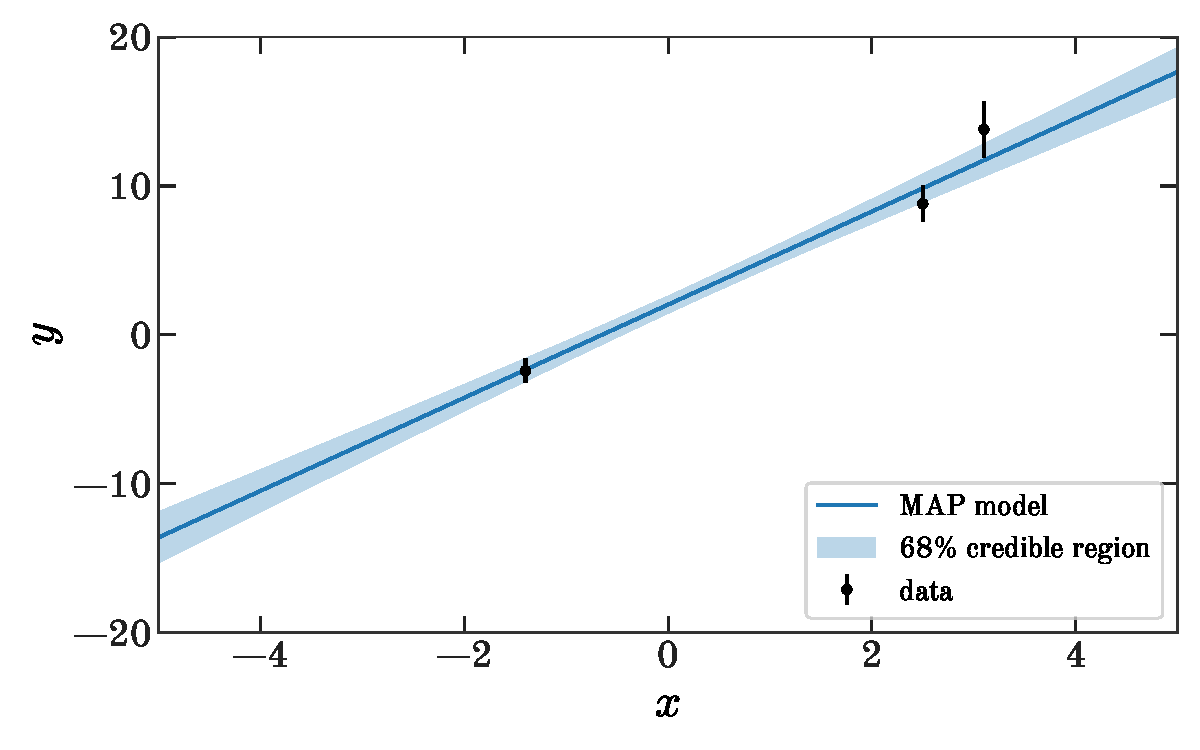
\includegraphics[width=0.7\textwidth]{exercise1.pdf}
  \caption{The solution to Exercise 1. The MAP parameter values were found using
  \equationname~\ref{eq:a}.}
  \label{fig:ex1}
\end{figure}

\subsection{Exercise 2: A model with linear and nonlinear parameters}

\paragraph{Problem:} We observe a set of data $(x_i, y_i)$ (indexed by $i$) with
known, Gaussian uncertainties in $y$, $\sigma_{y_i}$, and no uncertainty in $x$.
The parametric model we will use for this data is a generalized sinusoid with a
constant offset,
\begin{equation}
  % APW: I used greek here because a, b are used in expressions above...
  f(x \,;\, \alpha, \beta, \gamma, \omega) =
    \alpha\,\cos(\omega \, x) + \beta\,\sin(\omega \, x) + \gamma
\end{equation}
and we again assume we have Gaussian prior pdfs on all of the \emph{linear}
parameters $(\alpha, \beta, \gamma)$.
\todo{Set up this problem by stating some explicit Astro problems with this structure. Mention asteroseismology, if summing over frequency}
Here, we can no longer analytically express the posterior pdf because of the
nonlinear parameter $\omega$, but we can compute the marginal likelihood
(marginalizing over the linear parameters).

\tablename~\ref{tbl:data2} contains four data points, $(x_i, y_i,
\sigma_{y_i})$.
Assuming
\begin{align}
  (\mu_\alpha, \sigma_\alpha) &= (0, 5)\\
  (\mu_\beta, \sigma_\beta) &= (0, 5)\\
  (\mu_\gamma, \sigma_\gamma) &= (0, 10) ~ ,
\end{align}
compute the MAP parameter values $\va\T = (\alpha_{\rm MAP}, \beta_{\rm MAP},
\gamma_{\rm MAP})$.
Write a function to compute the design matrix and components ($\va, \tA, \vb, \tB$) of the factorization
 given a value of $\omega$.
Compute the marginal likelihood $p(\vy\given\omega)$.

% Generated with notebooks/Exercise2.ipynb
\begin{table}[t!]
  \footnotesize
  \begin{center}
    \begin{tabular}{c|c|c}
      $x$ & $y$ & $\sigma_y$ \\
      \hline
      $-1.2$ & 11.2 & 0.2 \\
      1.3 & 16.1 & 0.2 \\
      3.1 & 10.2 & 0.3 \\
      4.1 & 13.5 & 0.3
    \end{tabular}
    \caption{Simulated data used in Exercise 2
    (\href{https://raw.githubusercontent.com/davidwhogg/GaussianProductRefactor/master/notebooks/data2.csv}{link to data}). These data were generated with the true parameter values $(\alpha, \beta, \gamma, \omega) = (3.21, 2.44, 13.6, 1.27)$.
    \label{tbl:data2}}
  \end{center}
\end{table}

\section{Generalization: product of many Gaussians}
\label{sec:generalization}

A case that arises in some applications is that the
likelihood is made of multiple Gaussian terms, each of which is a
different linear combination of the linear parameters $\vtheta$.
That is, there are many data vectors $\vy_i$, each of which has size or length $N_i$,
and each of which has an expectation
set linearly by the parameters $\vtheta$ but through a different design matrix $\mM_i$.
Provided that the different data vectors $\vy_i$ are independently ``observed'' (that
is, they have independent noise draws), the total likelihood is just the product of
the individual-data-vector likelihoods.
That setup leads to the following problem:

\paragraph{Problem:}
Find $K$-vector $\va$, $K\times K$ variance tensor $\tA$, $N_i$-vectors $\vb_i$,
and $N_i\times N_i$ variance tensors $\tB_i$ such that
\begin{equation}\label{eq:genproblem}
\normal(\vtheta\given\vmu,\tLambda)\,\prod_i\normal(\vy_i\given\mM_i\cdot\vtheta,\tC_i)\,
 = \normal(\vtheta\given\va,\tA)\,\prod_i\normal(\vy_i\given\vb_i,\tB_i) ~ ,
\end{equation}
and such that $\va$, $\tA$, all the $\vb_i$, and all the $\tB_i$
don't depend on $\vtheta$ at all.
Note that
$\vtheta$ is a $K$-vector,
$\vmu$ is a $K$-vector,
$\tLambda$ is a $K\times K$ non-negative semi-definite variance tensor,
each $\vy_i$ is an $N_i$-vector,
each $\mM_i$ is a $N_i\times K$ matrix,
and
each $\tC_i$ is a $N_i\times N_i$ non-negative semi-definite variance tensor.

\paragraph{Solution:}
\hogg{BL: IS THIS SOLUTION CORRECT? I intuited it!}

\begin{equation}\label{eq:genA}
\tA\inv = \tLambda\inv + \sum_i\mM_i\T \cdot \tC_i\inv \cdot \mM_i
\end{equation}
\begin{equation}\label{eq:gena}
\va = \tA \cdot (\tLambda\inv \cdot \vmu + \sum_i\mM_i\T \cdot \tC_i\inv \cdot \vy_i)
\end{equation}
\begin{equation}\label{eq:genB}
\tB_i = \tC_i + \mM_i \cdot \tLambda \cdot \mM_i\T
\end{equation}
\begin{equation}\label{eq:genb}
\vb_i = \mM_i \cdot \vmu
~ .
\end{equation}

\paragraph{Argument, proof, or notes:}
\hogg{BL, please write stuff here! Also I think you are using $\tLambda_i$ when
  you mean to be using $\tC_i$.}

\hogg{BL: I think you should move the canonical-form discussion above to the ``solution notes'' part of Section~\ref{sec:problemsolution}; it is useful there too! And then you can just name-check it here in your commentary.}

For a fixed number of terms, the techniques from above (completing the square and detailed balance) could be used but become cumbersome. We will derive a general formula using \textit{the canonical form of Gaussian distributions}.
For a multivariate Gaussian $\normal(\vx\given\vm,\tLambda)$, the canonical form is
\begin{equation}
\normal^{\ -1}(\vx\given\veta, \tH) = \exp\left(\xi +  \veta^T\cdot\vx - \frac{1}{2}\vx^T \cdot\tH \cdot \vx\right)
~ ,
\end{equation}
The parameters are obtained by equating the canonical form with the standard form, $\tH = \tLambda^{\ -1}$, $\veta = \tH\cdot \vm = \tLambda^{-1}\cdot \vm$, and the normalization
$\xi = -\frac{1}{2}\left( d\log 2\pi -\log|\tH| + \veta^T \cdot \tH\inv\cdot \veta \right)$
with $d$ the dimensionality of $\vx$.

Equipped with the canonical form, it is easy to see that the product of any number of Gaussians will reduce to the product of two terms: one with all of the terms in $\veta$ and $\vx$, and the other one the normalization necessary to turn the first term into a valid canonical form. We will apply this idea to (\hogg{what}):
\begin{eqnarray}
\prod_i \normal( \mM_i\cdot\vtheta \given \vmu_i,\tLambda_i) &=& \prod_i \normal^{\ -1}( \mM_i\cdot\vtheta\given\veta_i, \tH_i) \\
&=&   \underbrace{\normal^{\ -1}(\vtheta\given\bar{\veta}, \bar{\tH})}_{ \normal(\vtheta\given\va,\tA) } \ \times \ \exp\left(\textstyle{\sum_i} \xi_i - \bar{\xi} \right)
\end{eqnarray}
naturally grouping the terms depending on $\vtheta$ and following the convention of the previous section.

The parameters of the individual Gaussians in canonical form are
\begin{eqnarray}
\veta_i &=& \tLambda_i^{-1} \cdot \vmu_i \\
\tH_i  &=& \tLambda_i^{-1}\\
\xi_i &=& -\frac{1}{2}\left( d_i \log 2\pi -\log|\tH_i| + \veta_i^T \cdot \tH_i\inv\cdot \veta_i \right)
\end{eqnarray}
where $d_i$ is the dimensionality of $\vmu_i$, and that of the total Gaussian are
\begin{eqnarray}
\bar{\veta} &=& \sum_i \mM_i \cdot \veta_i = \sum_i \mM_i \cdot  \tLambda_i^{-1} \cdot \vmu_i  \\
\bar{\tH} &=& \sum_i  \mM_i^T\cdot \tH_i\cdot \mM_i = \sum_i  \mM_i^T\cdot \tLambda_i^{-1}\cdot \mM_i \\
 \bar{\xi} &=&  -\frac{1}{2}\left( N\log 2\pi -\log|\bar{\tH} | + \bar{\veta}^T \cdot \bar{\tH}\inv\cdot \bar{\veta} \right)\\
\va &=&  \bar{\tH}^{-1} \bar{\xi} \\
\tA &=& \bar{\tH}^{-1}
\end{eqnarray}
where $N$ is the dimensionality of $\vtheta$.
Equipped with this result, we can re-derive the formulae of the previous sections.
We can again identify $\va$ as the maximum a posteriori value for $\vtheta$, and $\tA$ the associated Gaussian covariance.
Furthermore, the term $ \normal(\vtheta\given\va,\tA) $ reduces to one when marginalizing over $\vtheta$, and we are left with the marginalized likelihood, $ \exp\left(\textstyle{\sum_i} \xi_i - \bar{\xi} \right)$.

One culprit of this approach is that its implementation. Indeed, it involves inverting the individual covariances $\tLambda_i$, projecting them with $\mM_i$, in order to form $\bar{\tH}$ and  $\bar{\veta}$ and apply them onto each other to obtain $\va$, $\tA$ and $ \bar{\xi}$. Depending on the condition numbers of the square matrices, and the dimensionality of the projection matrices, applying those formulae may be numerically unstable. In practice, this could simply result from the noise levels in the data and how the model is projected from the parameters $\vtheta$ onto the data.
It is therefore highly recommended to apply those formulae with care, and verify the stability of the results.
If matrices with bad condition numbers are involved, one solution would be to apply the matrix inversion lemma. Unfortunately this would only apply to one term $\mM_i^T\cdot \tLambda_i^{-1}\cdot \mM_i$ at a time, and it may be necessary to apply it multiple times, resulting in long expressions (that lead to numerically stable results).
Since this is application-specific, we do not derive those expressions here.

\end{document}
